\documentclass[12pt,a4paper]{article}

\usepackage[utf8]{inputenc}
\usepackage[spanish]{babel}
\addto\captionsspanish{\renewcommand{\tablename}{Tabla}}
\usepackage{amsmath, amssymb}
\usepackage{graphicx}
\usepackage{geometry}
\usepackage{booktabs}
\usepackage{hyperref}
\usepackage{natbib}
\usepackage{caption}
\usepackage{float}
\usepackage{siunitx}
\usepackage{orcidlink}

\sisetup{output-decimal-marker={,}}
\geometry{margin=2.5cm}

\title{Análisis de la eficiencia del prensado mecánico y la extracción por solvente en la obtención de aceite de chía (\textit{Salvia hispanica} L.)}

\author{%
\parbox{\textwidth}{\centering
Cortese CM\textsuperscript{1}\orcidlink{0009-0002-2184-7991};\;
Fernández MB\textsuperscript{1,2,3}\orcidlink{0000-0001-6910-5474};\;
Capitani MI\textsuperscript{1,2}\orcidlink{0000-0001-5663-4537} \\[1em]
{\small
\textsuperscript{1}UNCPBA, Facultad de Ingeniería, Departamento de Ingeniería Química y Tecnología de los Alimentos, TECSE, Olavarría, Buenos Aires, Argentina. \\
\textsuperscript{2}CONICET - CCT Tandil, Tandil, Buenos Aires, Argentina. \\
\textsuperscript{3}CIFICEN, UNCPBA-CICPBA-CONICET, Olavarría, Buenos Aires, Argentina.
}
}
}

\date{}




\begin{document}

\maketitle

% --- Resumen ---
\renewcommand{\abstractname}{Resumen}
\begin{abstract}

Teniendo en cuenta la importancia entre la alimentación y la salud, es relevante el rol que cumplen los aceites vegetales fuente de ácidos grasos omega 3, 6 y 9. Entre ellos, las semillas de chía se destacan por su considerable aporte de omega 3. Por ello, en el presente trabajo se comparó el rendimiento de extracción de aceite de semillas de chía (\textit{Salvia hispanica} L.) al aplicar  dos procesos convencionales: prensado mecánico y extracción con solvente (\textit{n}-hexano) mediante equipo Soxhlet. Los resultados mostraron que la extracción con solvente presentó un rendimiento superior (32,2\% b.s.) respecto al prensado mecánico (24,2\% b.s.). Se discuten alternativas al empleo de \textit{n}-hexano, considerando aspectos de seguridad y sustentabilidad.
\end{abstract}

\vspace{0.5em}
\noindent\textbf{Palabras clave:} chía, aceite, rendimiento, prensado mecánico, extracción sólido-líquido, sustentabilidad
\vspace{1em}

% --- Secciones ---
\section{Introducción}

La semilla de chía (\textit{Salvia hispanica} L.) es una oleaginosa ancestral, utilizada por las civilizaciones maya y azteca como fuente alimentaria. En las últimas décadas, ha recobrado interés por su perfil nutricional excepcional, destacándose por un contenido lipídico cercano al 35\,\%, con aproximadamente un 65\,\% de ácidos grasos omega-3, principalmente ácido alfa-linolénico (ALA). Además, constituye una fuente natural de fibras solubles e insolubles, proteínas, vitaminas, minerales y antioxidantes \citep{ixtaina2011characterization}.

Gracias a esta composición, la chía es considerada un “alimento funcional”, ya que no solo contribuye a la nutrición humana, sino que también favorece el aumento del índice de saciedad y la prevención de enfermedades cardiovasculares, metabólicas, inflamatorias y neurodegenerativas. Su versatilidad ha impulsado su incorporación en diversas industrias: alimentaria, farmacéutica, nutracéutica y de nutrición animal, entre otras \citep{munoz2013chia}.

La obtención de aceites vegetales representa un proceso clave tanto en el ámbito industrial como en el alimentario. En particular, el aceite de chía ha despertado creciente interés por su alto contenido de ácidos grasos poliinsaturados y compuestos bioactivos. Para su extracción, se emplean principalmente dos metodologías: el prensado mecánico, que no requiere solventes y se considera más seguro desde el punto de vista ambiental y alimentario; y la extracción con solvente, que suele ofrecer mayores rendimientos pero implica consideraciones de seguridad y sustentabilidad.

El objetivo de este trabajo fue comparar los rendimientos de ambas técnicas aplicadas a semillas de chía, evaluando la eficiencia de cada proceso y la cantidad de aceite obtenida. Asimismo, se propone el uso de la herramienta Overleaf como soporte para la redacción colaborativa y profesional del presente documento.



\section{Materiales y Métodos}

\subsection{Muestra}

Se trabajó con semillas de chía (\textit{Salvia hispanica} L.) cedida por la empresa Dusen S.R.L. (Argentina). Las mismas se almacenaron bajo refrigeración (8°C) hasta su posterior uso.

\subsection{Determinación de humedad}

El contenido de humedad de la semilla se determinó mediante la Técnica Af 2-54 \citep{aocs1998}, donde 10 g de muestra fueron secados en estufa de circulación de aire a 130°C por un lapso de 3 h. La humedad del expeller fue determinada según Técnica Ba2a-38 \citep{aocs1998}, con 2 g de muestra secados a 130°C por 2 h. El porcentaje de humedad expresado en gramos de agua por cada 100 gramos de sólido seco (\% b.s.) se calculó según la Ecuación~\ref{eq:Humedad}.


\begin{equation}
\% \text{Humedad} = \frac{\text{Peso húmedo} - \text{Peso seco}}{\text{Peso húmedo}} \times 100
\label{eq:Humedad}
\end{equation}

\subsection{Métodos de extracción de aceite}

Se llevaron a cabo dos métodos de extracción de aceite. El primero consistió en un prensado mecánico utilizando una prensa helicoidal a escala piloto (IMEGEN) (Figura~\ref{fig:prensado}), que permitió obtener el expeller como subproducto sólido. El segundo método fue una extracción por solvente, empleando \textit{n}-hexano como disolvente en un equipo Soxhlet (Figura~\ref{fig:soxhlet}). Ambos procedimientos fueron comparados en términos de rendimiento y eficiencia.


\begin{figure}[H]
\centering
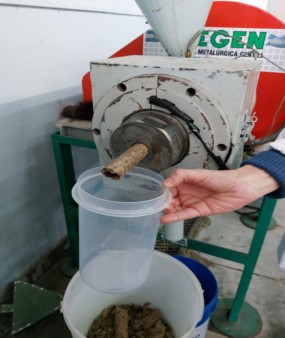
\includegraphics{Prensado.jpg}
\caption{Operación de prensado: salida de expeller}
\label{fig:prensado}
\end{figure}

\begin{figure}[H]
\centering
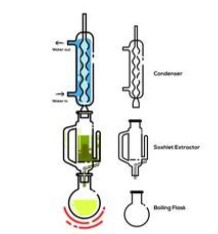
\includegraphics{Soxhlet.jpg}
\caption{Equipo extractor Soxhlet}
\label{fig:soxhlet}
\end{figure}

\subsection{Cálculo de rendimiento y eficiencia}

En todos los casos, el contenido de aceite se expresó como porcentaje en base seca (\% b.s.), calculado mediante la Ecuación~\ref{eq:aceite}. Esta fórmula se aplicó tanto para determinar el contenido total de aceite presente en la semilla como para estimar el aceite residual en el expeller obtenido tras el prensado.

Para establecer el rendimiento global de la prensa, fue necesario conocer ambos valores: el porcentaje de aceite total en la semilla y el porcentaje de aceite residual en el expeller. Estos datos se obtuvieron a partir de dos experiencias complementarias. En primer lugar, se realizó una extracción por solvente utilizando un equipo Soxhlet (Figura~\ref{fig:soxhlet}), lo que permitió cuantificar el contenido total de aceite de la semilla, considerado como el 100\% disponible. En segundo lugar, se llevó a cabo el prensado mecánico de una muestra independiente de semillas, obteniéndose el expeller como subproducto sólido (Figura~\ref{fig:prensado}). A partir de este expeller se determinó el contenido de aceite residual, también mediante la Ecuación~\ref{eq:aceite}.

Con ambos valores —contenido total de aceite en la semilla y aceite residual en el expeller— se aplicó la Ecuación~\ref{eq:rendimiento-global}, que permite calcular el rendimiento de extracción de aceite por prensado. Este rendimiento representa la eficiencia de la prensa en términos de porcentaje de aceite efectivamente extraído respecto al contenido total disponible en la semilla.

\begin{equation}
\% \text{Aceite (bs)} = \frac{\text{g de aceite}}{\text{Peso seco}} \times 100
\label{eq:aceite}
\end{equation}

\begin{equation}
\% \text{Rendimiento global} = \frac{X_{\text{semilla}} - X_{\text{expeller}}}{1 - X_{\text{expeller}}} \times 100
\label{eq:rendimiento-global}
\end{equation}

%\begin{equation}
%\% \text{Aceite extraído} = \frac{\text{Rendimiento expeller}}{\text{Rendimiento semilla}} \times 100
%\label{eq:aceite-extraido}
%\end{equation}

\subsection{Herramienta de soporte metodológico}

Se empleó Overleaf para la redacción técnica del documento, plataforma online basada en LaTeX (\citet{palma2023ciencia}). 


\section{Resultados}

Los contenidos de aceite correspondientes tanto a semilla como expeller se muestran a continuación en la Tabla~\ref{tbl:aceite}.

\begin{table}[H]
\centering
\caption{Contenido de aceite en semilla y harina residual del prensado mecánico}
\label{tbl:aceite}
\begin{tabular}{lc}
\toprule
\textbf{Muestra} & \textbf{\% Aceite (b.s.)} \\
\midrule
Semilla & 32,24 ± 0,64 \\
Harina  & 10,67 ± 0,07 \\
\bottomrule
\end{tabular}
\end{table}

La extracción con solvente mostró un rendimiento aproximadamente 8\,\% superior al prensado mecánico. A partir de los datos presentados en la Tabla~\ref{tbl:aceite}, y aplicando la Ecuación~\ref{eq:rendimiento-global}, se calculó que el rendimiento global de la operación por prensado fue del 24,15\%.
En la práctica industrial, suele emplearse un esquema combinado de prensado seguido de extracción con solvente para maximizar la recuperación de aceite. Sin embargo, el uso de \textit{n}-hexano presenta serias limitaciones: es inflamable, neurotóxico y genera riesgos de seguridad ambiental y ocupacional \citep{quimica_sostenible_2011}. Por ello, se discuten alternativas más seguras y sostenibles como el empleo de etanol, isopropanol o fluidos supercríticos \citep{rodriguez_2019, tornero_2015}.

\section{Conclusiones}

La extracción de aceite de chía mediante solvente resultó más eficiente que el prensado mecánico. No obstante, el uso de \textit{n}-hexano implica riesgos significativos, por lo que es necesario impulsar la adopción de tecnologías alternativas más seguras y sustentables, tales como el empleo de solventes renovables o fluidos supercríticos. Estos enfoques representan el futuro de la obtención de aceites vegetales de manera responsable con la salud y el medio ambiente.

\section*{Agradecimientos}

Los autores desean expresar su reconocimiento al Dr. Ing. Ricardo Raúl Palma (Universidad Nacional de Cuyo) por su impulso a la formación académica en redacción técnica y el uso de plataformas colaborativas como Overleaf. Su enfoque metodológico y pedagógico orientado a la innovación y la gestión tecnológica ha sido fuente de inspiración para este trabajo.



% --- Bibliografía ---
\bibliographystyle{plainnat}
\bibliography{Bibliografia}

\end{document}